%! suppress = LabelConvention
Asymptotic analysis, that classifies programs based on resource requirements, is the natural dual of studying complexity classes.
Since implicit computational complexity focuses on language-based characterizations, it produces analysis techniques for free.
It is a foundational hypothesis of this dissertation that theoretical ICC systems---with sufficient expressive power and an efficient evaluation strategy---enable concrete program analysis.
An analysis designed to evaluate a program's resource usage is called resource analysis.
Resource analysis is a subfield of static program analysis.

\subsubsection{Foundations of Static Program Analysis}\label{static-analysis-basics}

Static program analysis aims to answer questions about the runtime behaviors of programs.
The term \emph{static} means the analysis is conducted at compile-time on the program syntax and without execution.
The main motivations is to improve the performance characteristics of the generated executable~\cite{nielson2010,kennedy2001},
including detecting logical issues in the specification of the input program.
Foundational techniques include, \eg
type and effect systems;
control- and data-flow analyses;
abstract interpretation\index{abstract interpretation};
constraint-based, pointer, and inter-procedural analyses;
and fixed point algorithms~\cite{nielson2010,moller2023}.
Static program analysis is strongly practice-oriented and frequently materialized in automatic analyzers.
Real-world software development tools---like compilers, interactive development environments, and verifiers---rely on static analyses~\cite{livshits2015}.
A core challenges of static analysis concern precision and scalability of the techniques;
these topics are actively explored in research~\cite{schiebel2024}.

As a consequence of Rice's theorem~\cite{rice1953}\footnote{
Informally, Rice's theorem asserts that all interesting questions about the input/output behavior of programs written in a Turing-complete language are undecidable.}, it is impossible to construct a perfect program analyzer for a Turing-complete language.
All approaches must sacrifice something among soundness, completeness and termination~\cite{moller2024}.
Although seemingly discouraging, Rice's theorem should be viewed with optimism.
Since static program analysis is inherently undecidable, there is infinite opportunity in building increasingly precise approximations --
for inspiration see, \eg~\textcite{ding2023}.
The challenge is then to design analysis techniques that produce \emph{useful} answers \emph{efficiently} and \emph{often enough}.
This is colloquially called the \enquote{full employment theorem for static program analysis designers}~\cite[p. 4]{moller2023}.

Static analyzers typically evaluate programs against semantic properties\footnote{
Properties are introduced in~\autoref{verification-concepts}, but previewed here briefly.}.
More specifically, the focus is on \emph{safety properties}~\cite[p. 6]{moller2023},
which assert that something bad will not happen~\cite{lamport1977}.
Examples of safety properties include memory safety, absence of overflows, termination, and secure information flow (\cf~\autoref{if-elements}).
Safety properties have many applications in bug finding, program optimization, verification, \etc

\subsubsection{The Challenge of Approximation}\label{static-approx}

There are two broad categories of static analyzers~\cite{jourdan2015}.

\begin{itemize}

\item A \emph{bug finder} must discover potential errors that are hard to find by testing.
The analysis must be precise because excessive false alarms make the tool unusable.
The \emph{precision}\index{precision} of an analysis is the degree to which it avoids erroneous results~\cite{livshits2015}.
However, a bug finder offers no guarantee that all bugs will be found.

\item A program \emph{verifier} must establish that a given safety property holds with high confidence.
Critically, the analyzer must account for all execution paths.
If the analyzer reports no alarms, then it must be the case that the program is free of the errors tracked by the analyzer.

\end{itemize}

Obtaining the intended behavior depends on design choices, particularly on how the analysis approaches soundness and completeness.

\begin{figure}[t]
\centering
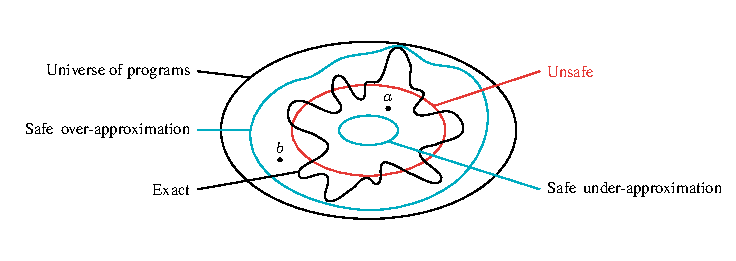
\includegraphics[width=\textwidth,keepaspectratio]{fig_approx}
\caption[Program analysis as an approximation.]{
Program analysis as an approximation -- an illustration inspired by~\textcite{steffen2020}.
The \textsc{exact} class of programs satisfying the analyzed property \(\phi\) is undecidable.
The program \(a\) satisfies \(\phi\), but the program \(b\) does not.
For an analyzer making a \textsc{safe under-approximation}, every accepted program truly satisfies \(\phi\), but would give an erroneous result on \(a\).
An analyzer making a \textsc{safe over-approximation} would accept \(a\) and \(b\), even though \(b\) does not satisfy \(\phi\).
However, an over-approximating analyzer never misses programs that satisfy \(\phi\).
Although an \textsc{unsafe} analysis can be justifiable in some cases,
interpreting its results is problematic because errors are not conservative.
}\label{fig:approx}
\end{figure}

\paragraph*{Soundness and completeness.}
A terminating static analyzer can either be sound or complete, but not both.
Soundness and completeness are terms from logic and not exclusive to static program analysis.
In logic, they carry the following meaning.
\begin{itemize}
\item A \emph{sound}\index{soundness} system guarantees that everything that is provable is true.
\item A \emph{complete}\index{completeness} system guarantees that everything that is true has a proof.
\end{itemize}
In the context of program analysis,
if a provably sound system reports that some property holds, then it must be true for the analyzed program.
A sound analyzer never misses a violation---\ie when a property does \underline{not} hold---but it may report an erroneous result for a satisfactory program~\cite{torlak2015}.
A complete analyzer detects all satisfactory programs, but also accepts cases where the tracked property does not truly hold.
The analysis approximation should be \emph{conservative}\index{conservative analysis}
whereby all errors occur on the \enquote{safe side} of the application domain~\cite[p. 5]{moller2023}.
Refer to Figures~\ref{fig:approx} and~\ref{fig:bug-verify} for examples.

\begin{figure}[t]
\centering
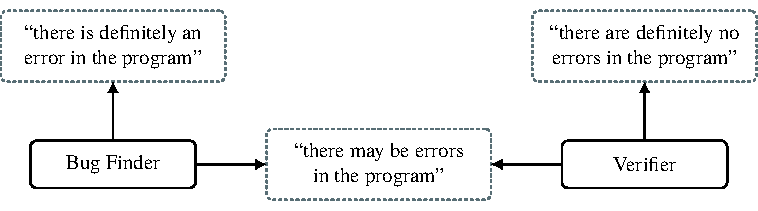
\includegraphics[width=.85\textwidth,keepaspectratio]{fig_bug-verifier}
\caption[Sound and incomplete bug detector vs. verifier]{
Behavior of sound and incomplete static analyzers: bug detector vs. verifier~\cite{moller2024}.
An \enquote{error} refers to some property tracked by the analyzer.}
\label{fig:bug-verify}
\end{figure}

To offer guarantees, a sound analyzer must overestimate the program behaviors.
It models all execution paths, including those that do not occur in any execution, like all branches of a conditional statement.
Soundness is challenging because it can render the analysis unscalable or imprecise to the point of being useless.
To maintain semantics, an optimizing analysis typically requires soundness~\cite[p. 5]{moller2023}.
A complete analyzer underestimates the program behaviors and thus errs on the other side.

\paragraph*{Soundiness.}
While academic literature widely emphasizes sound analyses, according to~\textcite{livshits2015}, strict soundness is a myth among realistic whole-program analyzers.
Practically-orientated static analyzers typically insist on Turing-completeness and termination,
but trade between soundness and completeness~\cite{moller2023,steffen2020}.
As an compromise, modern analyzers for real programming languages are often soundy.
A \emph{soundy}\index{soundy} analysis is as sound as possible, without excessively compromising precision or scalability~\cite{livshits2015}.

\subsubsection{Techniques of Resource Analysis}\label{resource-analysis}

Resource analysis\index{resource analysis}\footnote{
Also called \emph{cost analysis} when using an explicit \emph{cost measure}\index{cost measure}~\cite{albert2008}.
}---or (static/automatic) {complexity analysis}~\cite{rosendahl1989,leivant2013}---%
aims to obtain static information about the runtime {execution cost}\index{execution cost} of an analyzed program.
Such analysis naturally decomposes into two parts: one concerning the program's execution time and termination;
and the other change in the program's data-size~\cite{jones2009}.
Numerous techniques can be used to reason about such properties.

\begin{itemize}
\item Termination analyses tend to focus on values that are copied or decreased.
      Establishing termination is a critical aspect of correctness of recursive calls and commands.
      Termination analyses aim to discover conditions---like difference constraints~\cite{sinn2017},
      program-dependent well-founded orders on loops~\cite{lee2001}, or
      establishing that recursive reduction sequence are finite\footnote{
      Showing that every reduction sequence is finite is called the \emph{strong normalization} property~\cite[p. 36]{bertot2004}}---
      that guarantee termination.
      A specific technique for termination analysis, that originates from implicit computational complexity, is the size-change termination principle\index{size-change termination principle} of~\textcite{lee2001}.
\item Data-size analyses focus on memory consumption, estimating how large various variable values may become~\cite{lommen2023}.
      Obtaining bounds thus requires studying patterns of data-size changes during computation.
      In imperative programs, interesting data-size behaviors arise from counter increments and resets, particularly in loops~\cite{sinn2017,benamram2020}.
\end{itemize}

This dissertation is concerned with techniques of data-size analysis.
Among the specific and well-established techniques are automatic amortized\index{amortization} resource analysis and cost equation systems, presented briefly next.

\paragraph*{Automatic amortized resource analysis.}\index{AARA}
Amortized analysis\index{amortization} averages the time required to perform a sequence of operations over all the operations performed~\cite[p. 451]{cormen2009}.
It enables to show that the average cost of an operation is small, even if a single operation might be expensive.
Automatic amortized resource analysis (AARA)~\cite{hoffmann2022} builds on this idea to provide an automatic static technique for deriving arithmetic resource bounds.
In AARA, programs are bounded by amortized analysis\index{amortization}, which has the ability to account for amortization effects across operation sequences.
The analysis relies on inference rules, and derivation trees provide proofs of the resource bounds.
AARA originated from works in implicit computation complexity, particular from the contributions of Martin Hofmann~\cite{hoffmann2022}.
AARA-based techniques has been implemented on functional~\cite{hoffmann2017}, imperative~\cite{carbonneaux2015,carbonneaux2017}, and probabilistic~\cite{ngo2018} programming languages.

\paragraph*{Cost equation systems.}\index{cost equation system}
A \emph{cost equation system} (CES) (alternatively: cost relation system) is an abstract representation format of a program's resource cost~\cite{floresmontoya2017,albert2019}.
It consists of a set of cost equations, that are non-deterministic recurrence relations annotated with constraints, as shown in \autoref{lst:ces}~\cite{floresmontoya2014}.
The analyzing technique of cost equations is based on the seminal work of~\textcite{wegbreit1975}.
Such analysis operates in two phases.
The first phase extracts a set of equations that capture the program cost \wrt data-size and a parametric cost measure.
%\footnote{The generation phase converts the program's iteration constructs (loops and recursion) into recurrences,
%then infers size relations that approximate how the program's argument sizes vary.}.
This set can be regarded as recurrence relations, or as a kind of time-bound programs of~\textcite{rosendahl1989}.
The second phase searches for a non-recursive representation of the equations known as \emph{closed form}.
In most cases, it is not possible to find an exact solution, and the closed form provides an upper bound~\cite{albert2008}.
Cost equations deal with loops and recursion in a uniform manner,
but may have issues with multiphase loops and with programs with require complex termination proofs~\cite{floresmontoya2014}.

\begin{center}
\begin{minipage}{\textwidth}
\captionsetup{type=lstlisting}
\cesinputlisting{example.ces}
\captionof{lstlisting}[A cost equation system]{
A cost equation system representing an exponential function.
The term \pr|a(n)| is called the {head} and the rightward terms are the {body}.
The body terms represent costs and constraints.}
\label{lst:ces}
\end{minipage}
\end{center}

\subsubsection{A Sampler of Public Static Resource Analyzers}
\label{resource-analysis-tools}

The following list presents a small survey of automatic complexity analysis implementations, interpreted broadly.
It prioritizes tools that are open source or, at minimum, provide a public interface.
A comprehensive comparison of resource bounds computed by various tools is available online~\cite{flores_experiments}.

\begin{description}

\item[\href{https://costa.fdi.ucm.es/~costa/pubs/pubs.php}{{PUBS}}]
      \emph{\underline{P}ractical \underline{U}pper \underline{B}ounds} \underline{S}olver~\cite{albert2010}\index{PUBS}
      is a CES solver that computes closed form upper bounds for cost equation systems\index{cost equation system};
      specifically, for the \pr|entry| and all cost equations that depend on \pr|entry|.

\item[\href{https://aprove.informatik.rwth-aachen.de}{{AProVE}}]
      \emph{\underline{A}utomated \underline{Pro}gram \underline{V}erification \underline{E}nvironment}~\cite{giesl2016}\index{AProVE}
      produces termination proofs and complexity bounds for
      term rewrite systems,\index{term rewrite system},
      Java bytecode\index{bytecode},
      and programs written in
      C\index{C},
      Prolog\index{Prolog}, or
      Haskell\index{Haskell}.
      AProVE is a regular contestant in international tool competitions, including the
      \href{https://termination-portal.org/wiki/Termination_Competition}{Termination Competition}~\cite{giesl2019}
      and \href{https://sv-comp.sosy-lab.org/}{Competition on Software Verification} (SV-Comp)~\cite{beyer2022}.

\item[\href{https://github.com/aeflores/CoFloCo}{{CoFloCo}}]
      \emph{\underline{Co}ntrol \underline{Flo}w refinement of \underline{Co}st Relations}~\cite{floresmontoya2014}\index{CoFloCo}
      is an open-source analyzer and CES solver that infers symbolic upper and lower complexity bounds for CESs~\cite{flores-montoya2016}.
      CoFloCo is not bound to any particular programming language, but expects a input program translated to a CES~\cite{flores2016}.

\item[\href{https://github.com/academic-archive/pldi15}{C4B}]\cite{carbonneaux2015}\index{C4B}
      is an AARA-based analyzer of certified compositional resource bounds.
      It infers linear resource bounds on C-like programs by amortization\index{amortization} -- \autoref{tab:atva-compare}.

\item[\href{http://cl-informatik.uibk.ac.at/software/tct/}{TcT}]
       \emph{\underline{T}yrolean \underline{C}omplexity \underline{T}ool}~\cite{avanzini2016}\index{TcT}
       is a modular analyzer with front-ends to support term rewrite- and integer transition systems;
       high-order functional programs, and Java bytecode.
       The complexity problem and metric of interest are parametric.
       TcT has also competed in the Termination Competition.

\item[\href{https://koat.verify.rwth-aachen.de/cfr_mprf}{KoAT}]
       \emph{\underline{Ko}mplexitäts-\underline{A}nalyse-\underline{T}ool}~\cite{brockschmidt2016}\index{KoAT}
       is a complexity analyzer for computing time-, cost- and size bounds.
       As inputs, KoAT accepts Integer Programs (IPs)\index{integer program} and C integers programs that follow
       \href{https://termination-portal.org/wiki/C_Integer_Programs}{the grammar specification} of the Termination Competition -- \autoref{pc-expr}.

\item[\href{https://github.com/statycc/LQICM_On_C_Toy_Parser}{LQICM}]
      \emph{\underline{L}oop \underline{Q}uasi-\underline{I}nvariant \underline{C}hunk \underline{M}otion}~\cite{moyen20172}\index{LQICM}
       is a compile-time program optimization pass for C programs.
       It aims to peel (\cf~\autoref{loop-transforms}) inner loops to reduce program's time complexity.

\item[\href{https://www.raml.co/about}{RaML}]
       \emph{\underline{R}esource \underline{a}ware \underline{ML}}~\cite{hoffmann2017}\index{RaML}
       is an analyzer of worst-case upper bounds and best-case lower bounds of cost, for functional programs written in OCaml\index{OCaml}.
       The cost resource can be any quantity that is of interest.
       The RaML analysis is based on AARA and can produce precise amortized\index{amortization} bounds.

\item[\href{https://github.com/academic-archive/cav17-pastis}{Pastis}]\cite{carbonneaux2017,carbonneaux2018}
      is an AARA-based analyzer.
      It infers various resource bounds and size change information of programs expressed in LLVM bitcode (interprocedural CFGs).
      Additionally, it generates proof certificates that guarantee the validity of the inferred bounds.

\item[\href{http://cl-informatik.uibk.ac.at/users/zini/software/hosa/}{HoSA}]
      \emph{\underline{H}igher-\underline{O}rder \underline{S}ize \underline{A}nalysis}~\cite{avanzini2017}\index{HoSA}
      is a time complexity analyzer for higher-order functional programs written in a (generic) strongly typed functional programming language.
      The analysis technique is based on a type system and inference of sized types, and constraint solving.

\item[\href{https://github.com/davidnowak/cecoa}{Cecoa}]\cite{feree2018}\index{Cecoa}
     is a formal methods library based on implicit computational complexity.
     It enables creating proofs to show a program is poly-time computable\ccxi{p} -- \autoref{icc-formally}.

\item[\href{https://costa.fdi.ucm.es/maxcore/}{MaxCore}]%
      \emph{\underline{Max}-SMT termination analyzer + \underline{CO}st \underline{R}ecurrence \underline{E}quation solver}~\cite{albert2019}\index{MaxCore}
      is an upper bounds complexity analyzer for C programs\index{C}.
      The underlying technique is based on cost equations and termination analysis, and MaxCore uses CoFloCo and PUBS as back-end CES solvers.

\item[\href{https://www-sop.inria.fr/members/Martin.Avanzini/software/eco-imp/}{eco-imp}]\cite{avanzini2020}\index{eco-imp}
      computes expected cost bounds for programs written in a probabilistic imperative \textsc{pWhile} language.

\item[\href{https://gitlab.inria.fr/complexityparser/complexityparser}{ComplexityParser}]\cite{hainry2021}\index{ComplexityParser}
      is a complexity analyzer for Java\index{Java} programs.
      A typable program is guaranteed to run in polynomial time if the program terminates.
      The analyzer is based on~\cite{hainry2015} and~\cite{hainry2018}, discussed more in~\autoref{icc-sec}.

\item[\href{https://github.com/statycc/pymwp}{pymwp}]\cite{aubert2023b}\index{pymwp}
      is an implementation of the flow calculus of mwp-bounds.
      It is purely syntactical analysis of C\index{C} programs, to determine if the program's variable value growth is polynomially bounded in inputs -- \autoref{sec:atva}.

\item[\href{https://zenodo.org/records/10457566}{Quantitative probabilistic bounds}]\cite{chatterjee2024}
      analyzer computes tail and expectation bounds for programs written
      in a probabilistic imperative programming language \textsc{Prog}.

\end{description}

\subsubsection{Feature Considerations of ICC Techniques}\label{icc-feat}

\paragraph*{Soundness and completeness.}
In characterizing a complexity class,
a \emph{soundness} statement says that all programs of a given language, or those satisfying a restriction \(\mathcal{R}\), admit a certain complexity property, \ie compute functions in the target class.
A \emph{completeness} statement says that all functions of the corresponding functional complexity class can be programmed in this language~\cite{baillot2012}.
Alternatively, if \(\mathcal{R}\) is \emph{(extensionally) complete}, then for any problem in the complexity class, there exists a program in \(\mathcal{R}\) that decides it.
For instance, for polynomial time complexity, the soundness statement refers to a polynomial time evaluation of programs, whereas completeness refers to the class FP of functions computable in polynomial time~\cite{baillot2012}.
However, extensional completeness is of limited interest, as the goal is to validate as many interesting programs as possible.

ICC systems are typically proven sound \wrt the complexity class they characterize, whereby they are \emph{sound and incomplete} under-approximations of the target class~\cite[p. 125]{moyen2017}.
A sound and incomplete analysis admits false negatives, but guarantees the absence of false positives.
Complexity analysis can then give an erroneous result in the following way:
a developer writes a program that belongs to the intended complexity class,
but the program fails the analysis because it is not expressible in the ICC system.
Fixing the issue requires rewriting the program to satisfy the class membership restriction \(\mathcal{R}\).
Due to undecidability, it is impossible to completely avoid false negatives.
Stated differently, implicit complexity can decide non-trivial semantics properties of programs, but it will always exclude some programs that possess the property of interest.

\paragraph*{Input languages and expressive power.}
Extensional correspondence with complexity classes is usually not enough.
A programming language offering safety guarantees is plausible only
if it captures enough interesting and natural algorithms~\cite{baillot2012}.
On the other hand, sacrificing Turing-completeness allows developing an analysis that is \enquote{completely correct} about membership in a particular complexity class.
It requires defining a non-Turing-complete programming language and proving that it is sound and complete \wrt a particular complexity class.
%i.e., that their programs compute functions in \(\mathbb{C}\),
%and that for any problem in \(\mathbb{C}\), there is a program that solves it).
This sidesteps Rice's theorem, but cannot be \emph{intentionally} complete, since it will always exclude programs that yet belong to the targeted complexity class.
Correctly analysing a real world programming language is very difficult because of the large number of constructions allowed in it.

\begin{quotation}
\noindent We must understand all the difficulty because for a Turing-complete language for example the class of PTime programs is not recursively enumerable, and therefore an intentionally complete criterion would not be decidable~\cite[Sect. 4.1]{mogbil2012}.
\end{quotation}

\noindent For this reason, most research\footnote{
Among exceptions, quasi-interpretations~\cite{marion2000} considers a Turing-complete language.}
in implicit complexity techniques focuses on \enquote{toy languages}~\cite{moyen2017,rubiano17};
like term rewrite systems or the \textsc{Loop} language~\cite{kristiansen2005}.
% functional, imperative (oop, loops), flowchart, term rewriting,...
While such languages capture the core of mainstream programming languages, they are far from the rich constructs allowed in real languages.
%That limits the spread of implicit complexity-based techniques beyond academic circles and complicates rigorously assessing their potential.

\paragraph*{Analysis mechanics and obtained bounds.}
That ICC systems are designed to characterize a specific complexity classes has implications on the results they produce.
If they generate bounds, they are asymptotic (symbolic) bounds, rather than concrete bounds~\cite{baillot2019}.
An existing research direction in ICC concerns improving precision of obtained resource bounds~\cite{benamram2020}.
However, if the system is designed as a sound under-approximation, it can only provide upper bounds~\cite[p. 119]{moyen2017}.
A satisfactory program can be provided run-time complexity guarantee, but nothing is known of the runtime behavior of unsatisfactory programs.
ICC system is inherently restricted to analyzing programs whose sub-computations also satisfy the membership criterion of the target complexity class~\cite{baillot2019}.
On the other hand, unlike many other static analysis techniques,
ICC systems may not require establishing termination and avoid difficult control-flow analysis by abstraction and over-approximation~\cite{jones2009}.

\subsubsection{Prospects and Directions in ICC-Based Program Analysis}

There are two general strategies for implementing static analyses based on implicit computational complexity.
The first involves restricting the program syntax to guarantee all valid programs satisfy a desired property.
This is challenging for a software engineer since it may require writing programs in an unnatural way (though not all programs are written by humans).
However, if the program can be expressed in the given syntax, then the desired property is obtained \emph{for free}.

The second strategy allows a software engineer to write any program and performs program analysis \emph{aposteriori}.
Instead of requiring every program to be written using the restriction \(\mathcal{R}\),
we would test the adhesion of the program to the restriction \(\mathcal{R}\).
While this is more preferable for the program creator, such analysis is necessarily incomplete.
Some programs will be decided incorrectly and must be refactored to be acceptable to an analyzer.
Nonetheless, this strategy already has produced applications in~\textcite{moyen2016,moyen20172}.

%But implicit computational complexity is flexible enough to extend beyond complexity properties.
%Therefore, it can be leveraged in analysis of \emph{other} semantic properties.
%For example, it is possible to use ICC systems to develop static analysis tools.

Those research lines illustrates a shift from the design of ICC programming languages -- from pre-bounding all programs --
to the design of \emph{criteria} that may or may not be met by programs written in a Turing-complete programming language.
The first observation is crucial, considering that software engineers in general focus on much more tangible functional properties,
than complexity classes.
The second observation sends a mixed signal.
It seems that ICC will lose the originality of its approach by accepting to act as a post-filter on Turing-complete programming languages.
Let us not forget that by restricting the programming language itself, ICC offers the possibility of never having to run any analysis.

Compelling related examples of systems that provide properties by construction already exist.
The safe subset of the programming language Rust guarantees \eg memory safety and deadlock freedom by design.
Strongly normalizing interactive theorem provers require \emph{structural} fixed point termination~\cite{bertot2004}.
In return, every valid programs is known to terminate.
Although a software engineer cannot write every program, if they accept the restriction, they receive the termination guarantee for free.
Conceivably, implicit computational complexity techniques can provide similar \emph{X-by-Construction}\index{X-by-Construction}~\cite{terbeek2018} guarantees.
